\chapter{Знакомство с окном}\label{ch:okno}

\textbf{Что вы узнаете:} из чего состоит окно Litebee IDE, как запустить готовое шоу и где находится красная кнопка.

\section{Что мы делаем}

\textbf{Шоу дронов} — это программа для нескольких дронов сразу. У каждого дрона своя короткая программа из шагов: откалибровался, взлетел, зажёг свет, перелетел в другую клетку, сел. Мы пишем её на Python в обычном текстовом файле. Слово \textbf{симулятор} значит окно Litebee IDE: оно читает файл шоу и показывает карту с летающими дронами, временную ленту и список проверок.

Файл не вычисляет ничего сложного. Он просто \emph{записывает шаги}, а симулятор их проигрывает. Настоящий дрон нельзя перезапустить после ошибки, поэтому сначала шоу проверяют на экране.

\section{Верхняя панель}

\begin{figure}[H]
  \centering
  \fbox{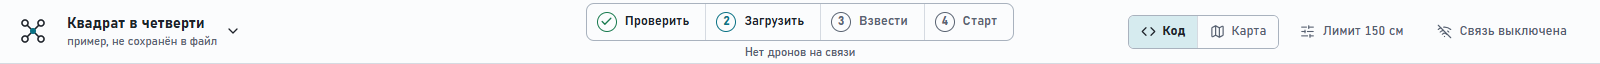
\includegraphics[width=\dimexpr\textwidth-2\fboxsep-2\fboxrule\relax]{figures/c_top.png}}
  \caption{Верхняя панель. Слева название проекта, в центре цепочка из четырёх кнопок, справа переключатель «Код / Карта», лимит высоты и состояние связи.}\label{fig:top}
\end{figure}

\begin{itemize}
  \item \textbf{Цепочка} \knopka{Проверить}, \knopka{Загрузить}, \knopka{Взвести}, \knopka{Старт}. Первая кнопка проверяет шоу на экране, остальные три нужны только для настоящих дронов (урок~\ref{ch:k-dronu}). Под цепочкой одна строка подсказки: что можно сделать сейчас.
  \item \textbf{Код} и \textbf{Карта}: два вида окна.
  \item \textbf{Лимит 150 см}: самая большая разрешённая высота.
  \item \textbf{Связь}: если дронов нет, здесь написано «Связь выключена». Для уроков связь не нужна.
\end{itemize}

\section{Код}

\begin{figure}[H]
  \centering
  \fbox{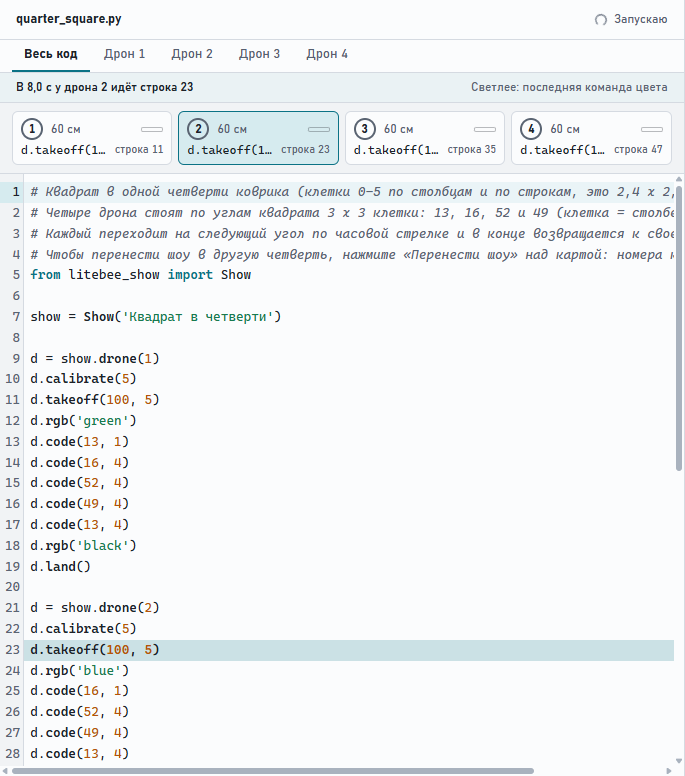
\includegraphics[width=0.62\textwidth]{figures/c_code.png}}
  \caption{Режим «Код». Вверху файл и состояние запуска, ниже вкладки по дронам, карточки дронов и код. Подсвеченная строка — та, что выполняется в выбранный момент.}\label{fig:code}
\end{figure}

В режиме \knopka{Код} виден текст шоу. Над ним вкладки: \knopka{Весь код} и по одной на каждого дрона. Под вкладками карточки дронов: на карточке номер, высота и цвет светодиода. Когда вы двигаете время, в коде подсвечивается строка, которая выполняется прямо сейчас.

\section{Карта}

\begin{figure}[H]
  \centering
  \fbox{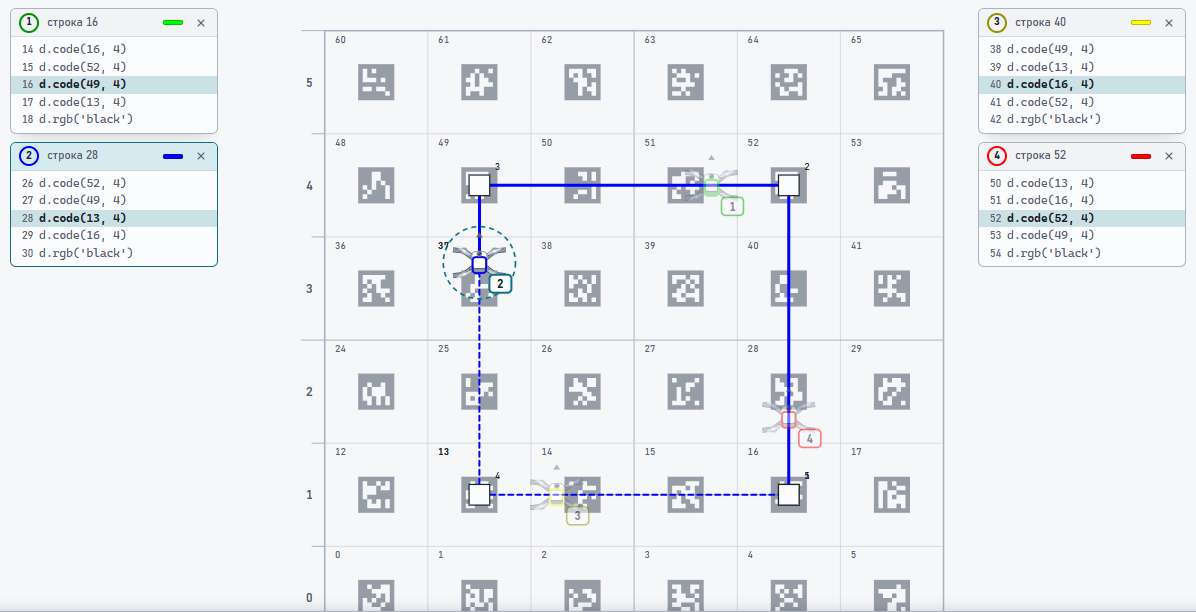
\includegraphics[width=\dimexpr\textwidth-2\fboxsep-2\fboxrule\relax]{figures/c_map.png}}
  \caption{Режим «Карта»: коврик сверху, дроны и их пути. По бокам окна с кодом каждого дрона, светлая строка — шаг, который идёт сейчас.}\label{fig:map}
\end{figure}

В режиме \knopka{Карта} в центре коврик: клетки с номерами и метками, дроны, их пути. Слева кружки с номерами дронов: щелчок выбирает дрона. Над картой выбор \knopka{Область} (весь коврик или одна четверть) и кнопка \knopka{Перенести шоу} (урок~\ref{ch:chetverti}).

\section{Время}

\begin{figure}[H]
  \centering
  \fbox{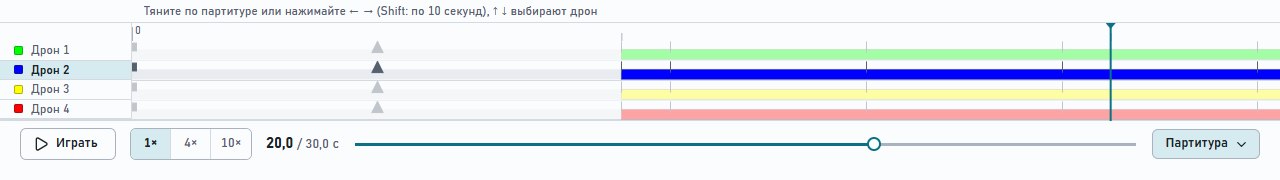
\includegraphics[width=\dimexpr\textwidth-2\fboxsep-2\fboxrule\relax]{figures/c_cue.png}}
  \caption{Панель времени и партитура. Внизу кнопка «Играть», скорость, время и ползунок; выше полосы дронов.}\label{fig:cue}
\end{figure}

Внизу окна: кнопка \knopka{Играть}, скорость (1$\times$, 4$\times$, 10$\times$), число вида «8,0 / 30,0 с» (сейчас и всего) и ползунок. Кнопка \knopka{Партитура} раскрывает полосы дронов. О них подробно в уроке~\ref{ch:partitura}.

\section{Красная кнопка}

В правом нижнем углу всегда видна красная кнопка \knopka{Аварийная посадка}. Ей соответствует клавиша \klavisha{Esc}. Она посылает команду посадки всем дронам на связи. Пока дронов нет, она просто останавливает симуляцию.

\begin{opasno}
Красная кнопка и \klavisha{Esc} работают в любой момент. Перед настоящим полётом убедитесь, что знаете, где она, и что рука может до неё дотянуться.
\end{opasno}

\begin{probuy}
  \item Откройте пример \knopka{Квадрат} (файл \texttt{quarter\_square}) и нажмите \knopka{Играть}. Сколько секунд длится шоу?
  \item Остановите время и посмотрите карточки дронов. Какого цвета светодиод у дрона 3?
  \item Выберите дрона 4 щелчком по кружку. Какая клетка у него стартовая?
  \item Нажмите \klavisha{Esc}. Что написано в сообщении?
\end{probuy}
\otvety{1}
